The deterministic event-based calculator is capable of computing losses and loss statistics for a single event for a collection of assets. The event is repeated many times to model the variation in the inter-event variability and for each event, a ground motion field is generated taking into account the intra-event variability (and possibly the spatial correlation of the latter). Figure \ref{fig:Scheme_deter_calc}  presents the deterministic event-based risk calculation workflow.

\begin{figure}[ht]
\centering
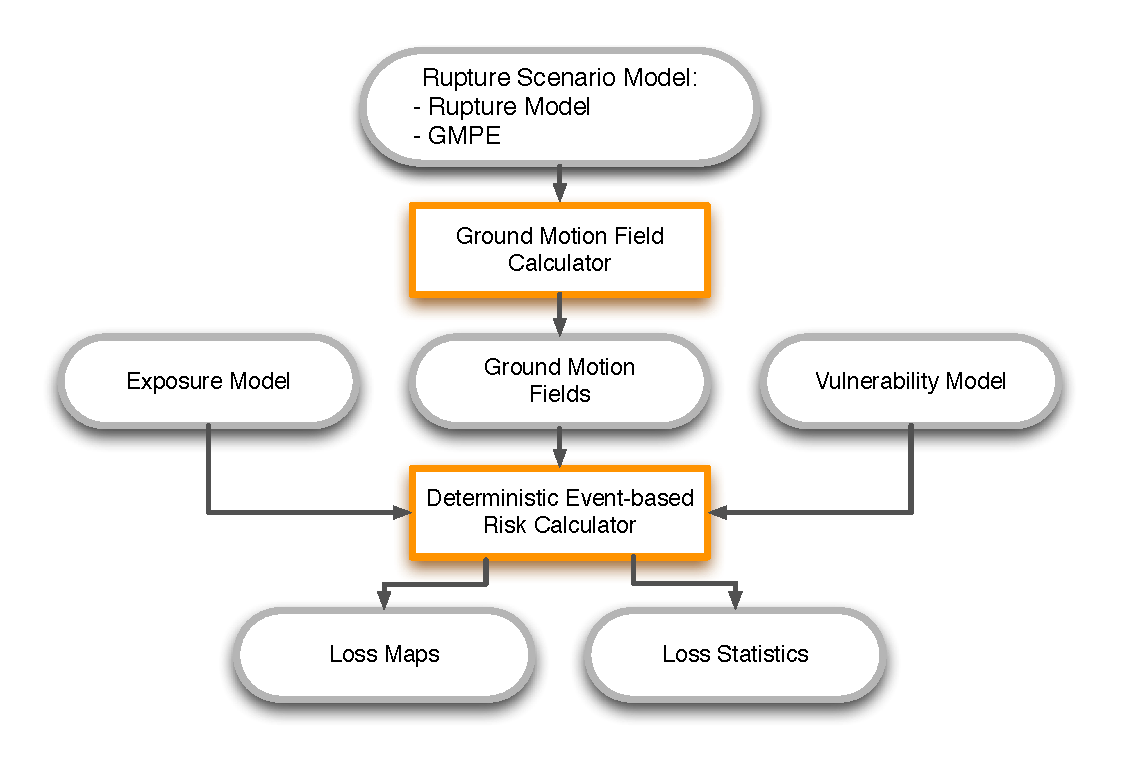
\includegraphics[width=9cm,height=9cm]{./Figures/Part_Risk/Scheme_Deter_calc.eps}
\caption{Workflow of the deterministic event-based risk calculator.}
\label{fig:Scheme_deter_calc}
\end{figure}


\section{Description}
For each ground motion field, the intensity measure level at a given site is combined with a vulnerability function to randomly sample a loss ratio for each asset typology contained in the exposure model. These loss ratios that are sampled for a given typology at different locations are considered to be independent or fully correlated, knowing that the reality is likely to lie somewhere in between these two assumptions. Using these results, the mean and standard deviation of loss ratio across all events can be calculated. Loss ratios are converted into losses by multiplying by the value of the asset given in the exposure model. For this method, it is possible to aggregate the losses throughout the region and to compute the standard deviation of the aggregated loss. 

\section{Calculation workflow}

To compute the mean loss:

\begin{enumerate}
\item For each ground motion field, the intensity measure level at the location of the asset is used to derived the mean loss ratio and associated coefficient of variation from the vulnerability function. Since currently the vulnerability functions are being defined in a discrete way, it is quite probable that the intensity measure level provided by the ground motion field is not contained in the vulnerability function. In these cases, linear interpolation methods are being employed to derive the mean loss ratio at the intensity measure level of interest. Once these two parameters are known, the sampling of the loss ratio is done following the probabilistic distribution of the respective vulnerability function, as described bellow:

\begin{equation}
\log{LR_n} = \mu + \epsilon\sigma
\end{equation}

Where $\mu$ and $\sigma$ stand for the mean and standard deviation of the logarithm of the loss ratios respectively and $\epsilon$ is a term that has a standard normal distribution with a zero mean and a standard deviation of one.  

The method used to sample this parameter can follow two approaches depending on whether the correlation between the vulnerability of similar asset typologies is to be considered or not:

\begin{itemize}

\item Perfectly correlated: the term $\epsilon$ is randomly sampled once for the first asset and this result is used to derive the loss ratio for all the assets of the same typology. 

\item Uncorrelated: the term $\epsilon$ is always randomly sampled for each asset and therefore the correlation between the vulnerability of the assets is ignored.

\end{itemize}

It is expected that the true level of correlation lies somewhere between these two assumptions, and thus they provide boundaries to the expected output. 


\item The mean loss ratio for each asset across all possible simulations of the deterministic event can be calculated through the formula:

\begin{equation}
LR=\frac{\sum^m_{n=1}LR_n|IML}{m}
\end{equation}

Where $m$ stands for the number of ground motion fields simulated.

\item The mean loss can then be derived by multiplying the mean loss ratio by the value of the asset contained in the exposure model file.

\end{enumerate}

To compute the standard deviation of the loss:

\begin{enumerate}

\item In order to compute the uncertainty, the engine takes the set of loss ratios for each asset, and computes the associated standard deviation using the classical formula:

\begin{equation}
SD[LR]=\sqrt{  \frac{1}{m}\sum_{n=1}^m{(LR_n-E[LR])^2} }
\end{equation}

Where $E[LR]$ stands for the mean loss ratio computed previously.

\item The standard deviation of the absolute loss can finally be computed by multiplying the standard deviation of the loss ratio by the value of the respective asset.

\end{enumerate}

